
$ABCDEFGH$ est un parallélépipède rectangle. On donne

$FE=12~$cm, $FG=9$~cm,
$FB=3$~cm, $FN=4$~cm et 
$FM=3$~cm
\begin{enumerate}
\item Construis la face $EFGH$ en vraie grandeur.
\item Construis un patron de ce parallélépipède rectangle $ABCDEFGH$.
\item Calcule la longueur $MN$.
\item Calcule l'aire du triangle $FMN$.
\item Calcule la longueur $EG$ puis déduis-en la longueur $EC$.
\end{enumerate}
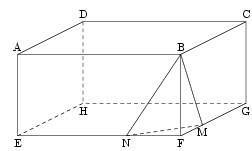
\includegraphics[scale=1]{RepS-exo1.png} 

